% -*- latex -*-
%%%%%%%%%%%%%%%%%%%%%%%%%%%%%%%%%%%%%%%%%%%%%%%%%%%%%%%%%%%%%%%%
%%%%%%%%%%%%%%%%%%%%%%%%%%%%%%%%%%%%%%%%%%%%%%%%%%%%%%%%%%%%%%%%
%%%%
%%%% This text file is part of the source of 
%%%% `Parallel Programming in MPI and OpenMP'
%%%% by Victor Eijkhout, copyright 2012-2020
%%%%
%%%% tau.tex : tutorial about tracing with TAU
%%%%
%%%%%%%%%%%%%%%%%%%%%%%%%%%%%%%%%%%%%%%%%%%%%%%%%%%%%%%%%%%%%%%%
%%%%%%%%%%%%%%%%%%%%%%%%%%%%%%%%%%%%%%%%%%%%%%%%%%%%%%%%%%%%%%%%

\Level 0 {TAU profiling and tracing}
\index{TAU|(}

TAU~\url{http://www.cs.uoregon.edu/Research/tau/home.php} is a utility
for profiling and tracing your parallel programs. Profiling is the
gathering and displaying of bulk statistics, for instance showing you
which routines take the most time, or whether communication takes a
large portion of your runtime. When you get concerned about
performance, a good profiling tool is indispensible.

Tracing is the construction and displaying of time-dependent
information on  your program run, for instance showing you if one
process lags behind others. For understanding a program's behaviour,
and the reasons behind profiling statistics, a tracing tool can be
very insightful.

\Level 1 {Workflow}

\Level 2 {Instrumentation}

Unlike such tools as \indexterm{VTune} which profile your binary as-is,
TAU works by adding \indexterm{instrumentation} to your code: in
effect it is a source-to-source translator that takes your code and
turns it into one that generates run-time statistics.

This instrumentation is largely done for you; you mostly need to recompile
your code with a script that does the source-to-source translation,
and subsequently compiles that instrumented code.
You could for instance have the following in your makefile:
\begin{verbatim}
ifdef TACC_TAU_DIR
  CC = tau_cc.sh
else
  CC = mpicc
endif

% : %.c
<TAB>${CC} -o $@ $^
\end{verbatim}
If TAU is loaded (which we detect here by checking for the environment variable
\indextermtt{TACC_TAU_DIR}), we define the \indextermtt{CC} variable as
one of the TAU compilation scripts; otherwise we set it to a regular MPI compiler.

\begin{istc}
To use \emph{TAU} on \emph{TACC}\index{TAU!on TACC resources} resources,
do \n{module load tau}.
\end{istc}

\Level 2 {Running}

You can now run your instrumented code;
trace/profile output will be written to file 
if environment variables \indextermtt{TAU_PROFILE} and/or \indextermtt{TAU_TRACE} are set:
\begin{verbatim}
export TAU_PROFILE=1
export TAU_TRACE=1
\end{verbatim}

A TAU run can generate many files: typically at least one per process.
It is therefore advisabe to create a directory for your tracing and profiling
information. You declare them to TAU by setting the environment variables
\indextermtt{PROFILEDIR} and \indextermtt{TRACEDIR}.
\begin{verbatim}
mkdir tau_trace
mkdir tau_profile
export PROFILEDIR=tau_profile
export TRACEDIR=tau_trace
\end{verbatim}

The actual program invocation is then unchanged:
\begin{verbatim}
mpirun -np 26 myprogram
\end{verbatim}

\begin{tacc}
At TACC, use \indextermtt{ibrun} without a processor count;
the count is derived from the queue submission parameters.
\end{tacc}

While this example uses two separate directories, there is no
harm in using the same for both.

\Level 2 {Output}

The tracing/profiling information is spread over many files, and hard to read as such.
Therefore, you need some further programs to consolidate and display the information.

You view profiling information with \indextermtt{paraprof}
\begin{verbatim}
paraprof tau_profile
\end{verbatim}
Viewing the traces takes a few steps:
\begin{verbatim}
cd tau_trace
rm -f tau.trc tau.edf
tau_treemerge.pl
tau2slog2 tau.trc tau.edf -o yourprogram.slog2 
\end{verbatim}
The \n{slog2} file can then be viewed with \indextermtt{jumpshot}:
\begin{verbatim}
jumpshot yourprogram.slog2
\end{verbatim}

\Level 1 {Sample output}

\begin{figure}[ht]
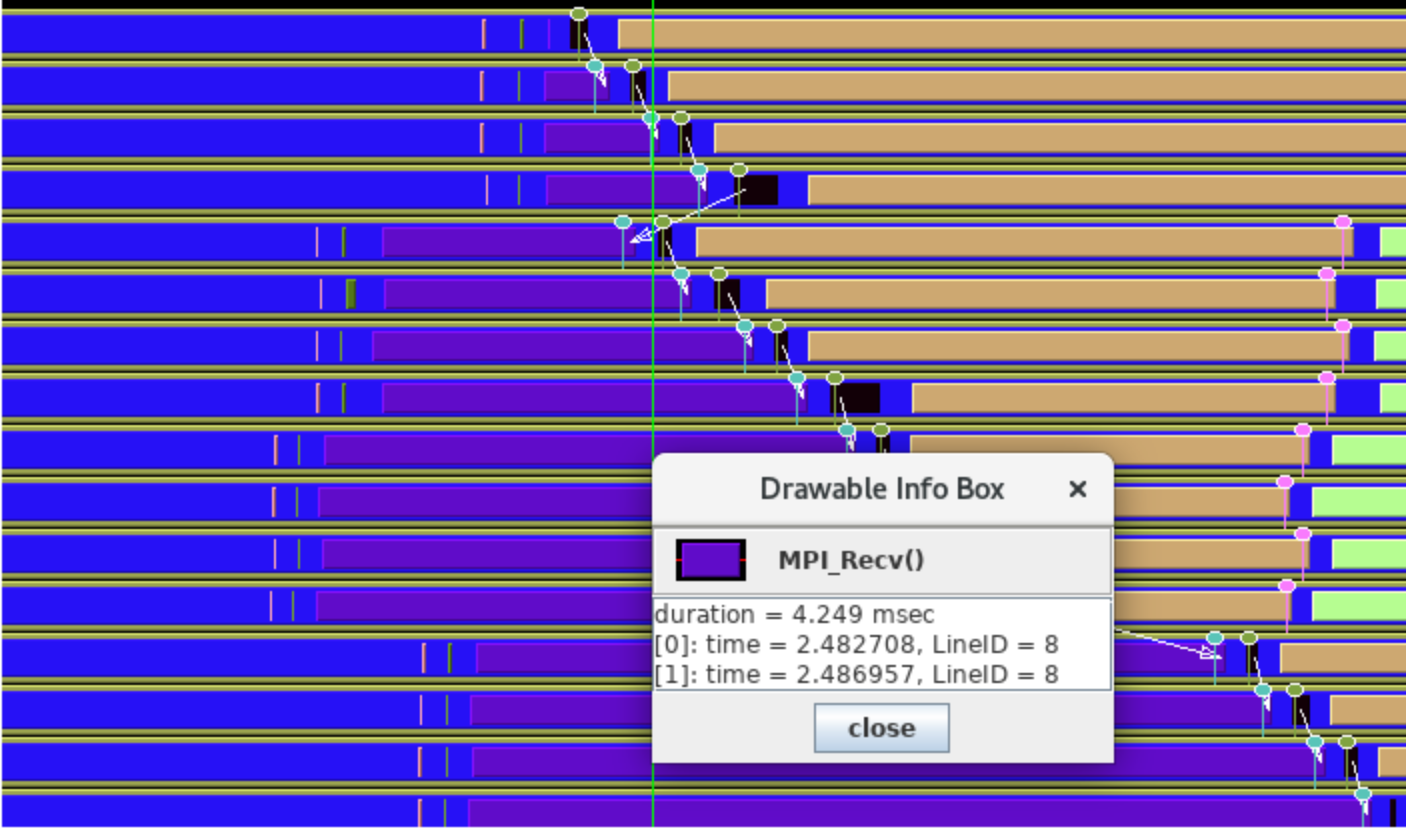
\includegraphics{tau-bucketblock}
\caption{Trace of a bucket brigade broadcast}
\label{fig:tau-bucketblock}
\end{figure}

%% \begin{figure}[ht]
%% 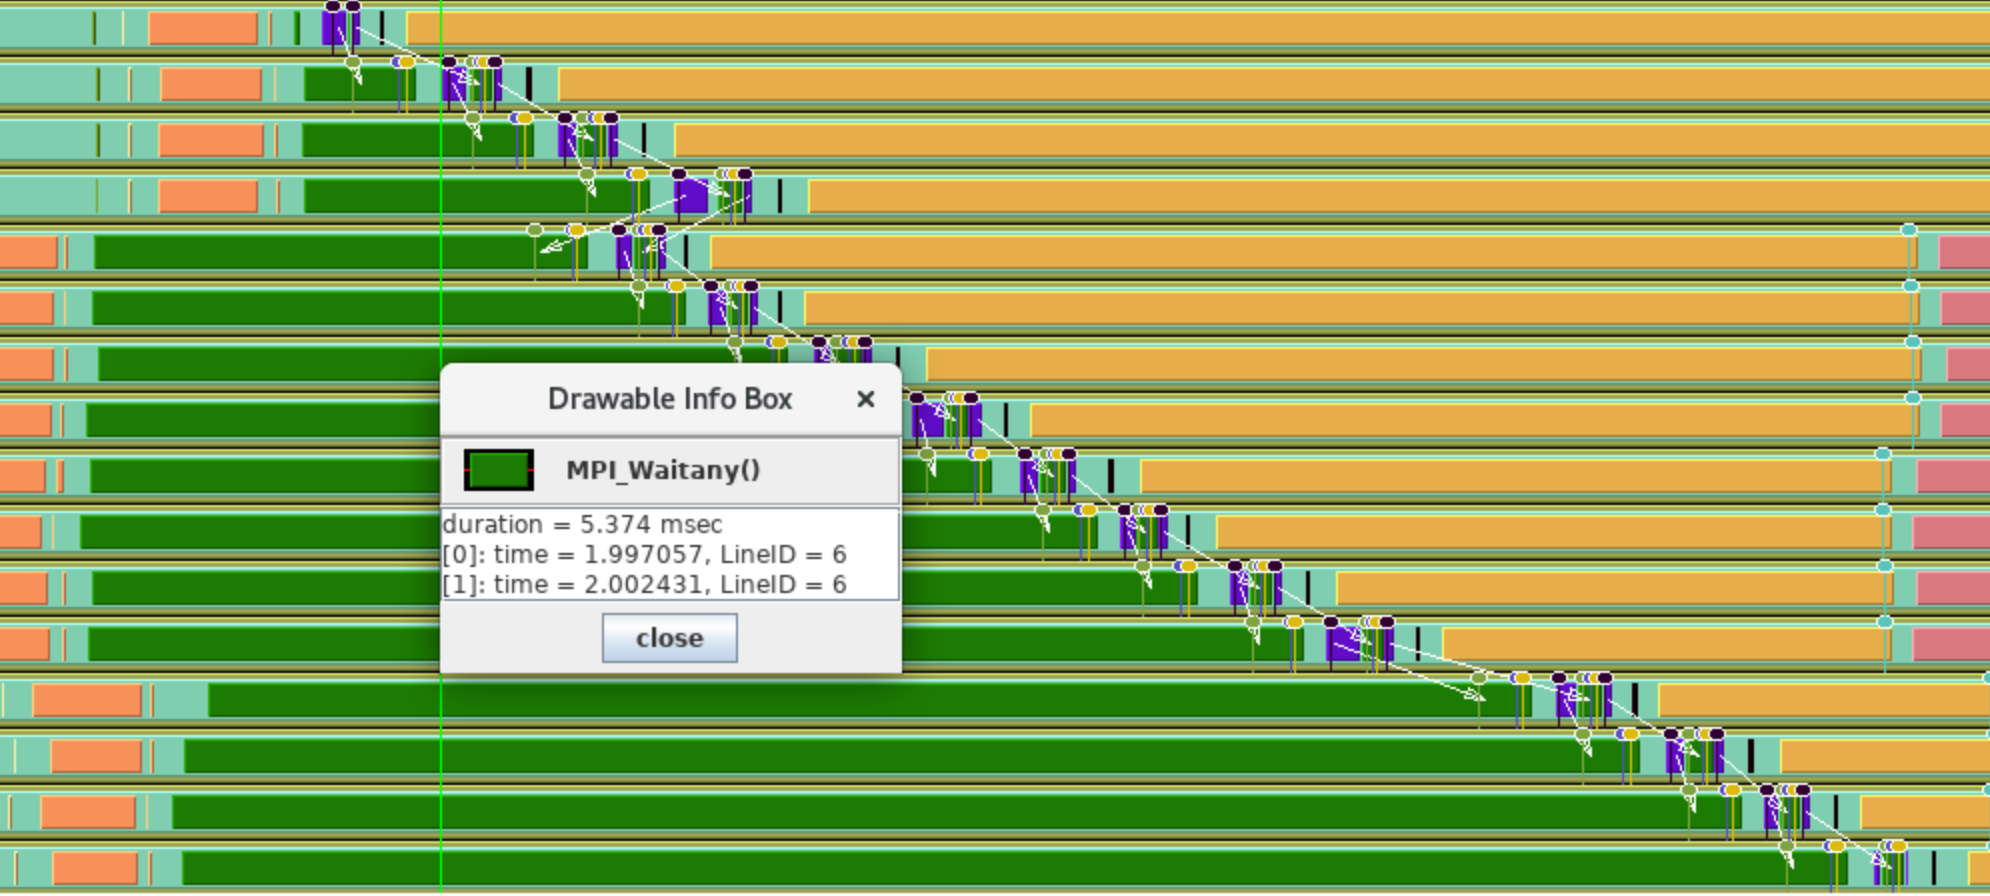
\includegraphics{tau-bucketpipe}
%% \caption{Trace of a pipelined bucket brigade broadcast}
%% \label{fig:tau-bucketpipe}
%% \end{figure}

Consider a very simple broadcast, executed by each processor (except for the first)
receiving data from its predecessor and sending it to its successor.
\begin{lstlisting}
int sendto =
    ( procno<nprocs-1 ? procno+1 : MPI_PROC_NULL )
    ;
int recvfrom =
    ( procno>0 ? procno-1 : MPI_PROC_NULL )
    ;

MPI_Recv( leftdata,1,MPI_DOUBLE,recvfrom,0,comm,MPI_STATUS_IGNORE);
myvalue = leftdata
MPI_Send( myvalue,1,MPI_DOUBLE,sendto,0,comm);
\end{lstlisting}

Figure~\ref{fig:tau-bucketblock} illustrates this on 4~nodes with 4~processes each.
\begin{itemize}
\item You see all processes posting a receive pretty much simultaneously;
\item but the conclusion of the receives happens in sequence.
\end{itemize}

\index{TAU|)}
